% SC4051 --- Chapter 4: Consensus (0->100)
\chapter{Consensus: Paxos, Raft and Byzantine Agreement}
\label{ch:consensus}

\begin{quote}
\emph{``Consensus is the distributed equivalent of agreeing on what time it is when no one has a correct watch.''} --- Barbara Liskov. Without agreement on order, replicas diverge; with it, they can act as one.
\end{quote}

\noindent\fbox{\parbox{\dimexpr\linewidth-2\fboxsep-2\fboxrule}{%
\textbf{From zero: why agreement is hard.} We build from a simple majority vote, show why naive voting fails under asynchrony and crashes, analyse Paxos and its understandable successor Raft, then extend to Byzantine faults. Runnable Python illustrates the core logic.}}
\vspace{0.4em}

\section*{Learning Outcomes}
After this chapter you will be able to:
\begin{enumerate}[label=(L\arabic*)]
    \item define consensus (agreement, validity, termination) and state FLP impossibility;
    \item trace Paxos prepare/promise/propose/accept and explain why a majority quorum suffices;
    \item describe Raft leader election, log replication and commitment rules;
    \item compare Paxos and Raft on understandability, liveness and leader transfer;
    \item explain PBFT phases and the $n\ge 3f+1$ bound for Byzantine agreement.
\end{enumerate}

% ============================================================
\section{The Consensus Problem and FLP}
\label{sec:consensus-def}
$n$ processes each propose a value; they must decide on one value satisfying:
\begin{description}[leftmargin=1.2em,style=nextline]
    \item[Agreement] No two correct processes decide differently.
    \item[Validity] If all propose $v$ then $v$ is decided (some forms: decided value was proposed by someone).
    \item[Termination] Every correct process eventually decides.
\end{description}
This looks easy---take a majority vote. But messages can be delayed and processes can crash. The celebrated FLP result (Fischer--Lynch--Paterson, 1985) proves:

\begin{theorem}[FLP impossibility]
No deterministic algorithm solves consensus in an asynchronous system with even one crash failure.
\end{theorem}

Consequence: every practical consensus algorithm either uses randomness or timing assumptions (timeouts, partial synchrony) to circumvent FLP. Paxos and Raft assume partial synchrony: the network is async but eventually timely enough for a leader to make progress.

% ============================================================
\section{Paxos: Single-Decree and Multi-Paxos}
\label{sec:paxos}
Paxos (Lamport, 1989/1998) has three roles: proposers, acceptors and learners. A value is \emph{chosen} when a majority of acceptors accept it. Two phases:

\paragraph{Phase 1 (Prepare).} Proposer picks ballot $b$ higher than any seen and sends $\langle prepare,b\rangle$ to a majority. Each acceptor that has not promised a higher ballot replies with $\langle promise,b, (b_{max},v_{max})\rangle$ (its highest accepted ballot/value, if any) and promises to ignore lower ballots.

\paragraph{Phase 2 (Accept).} Proposer collects promises from a majority. If any acceptor reported a value, the proposer must propose the value with the highest $b_{max}$ among them; otherwise it may propose its own. It sends $\langle accept,b,v\rangle$. Acceptors accept if they have not promised higher. When a majority accepts, $v$ is chosen.

Safety hinges on quorum intersection: any two majorities overlap, so if $v$ is chosen at ballot $b$, every higher ballot's Phase~1 will see $v$ and be forced to propose it.

\begin{figure}[h]
\centering
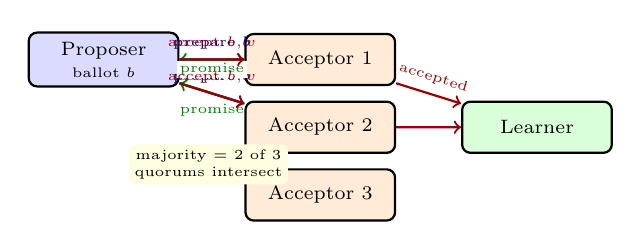
\begin{tikzpicture}[scale=0.86, every node/.style={font=\scriptsize},
  role/.style={draw,rounded corners=3pt,minimum width=1.9cm,minimum height=0.65cm,align=center,thick}]
\node[role,fill=blue!14] (prop) at (0,2.2) {Proposer\\{\tiny ballot $b$}};
\node[role,fill=orange!16] (acc1) at (3.2,2.2) {Acceptor 1};
\node[role,fill=orange!16] (acc2) at (3.2,1.2) {Acceptor 2};
\node[role,fill=orange!16] (acc3) at (3.2,0.2) {Acceptor 3};
\node[role,fill=green!15] (learn) at (6.4,1.2) {Learner};
\draw[->,thick,blue!60!black] (prop) -- (acc1) node[midway,above,font=\tiny] {prepare $b$};
\draw[->,thick,blue!60!black] (prop) -- (acc2) node[midway,above,font=\tiny] {prepare $b$};
\draw[<-,thick,green!50!black] (prop) -- (acc1) node[midway,below,font=\tiny,fill=white,inner sep=1pt] {promise};
\draw[<-,thick,green!50!black] (prop) -- (acc2) node[midway,below,font=\tiny] {promise};
\draw[->,thick,red!60!black] (prop) -- (acc1) node[midway,above,font=\tiny] {accept $b,v$};
\draw[->,thick,red!60!black] (prop) -- (acc2) node[midway,above,font=\tiny] {accept $b,v$};
\draw[->,thick,red!60!black] (acc1) -- (learn) node[midway,above,sloped,font=\tiny] {accepted};
\draw[->,thick,red!60!black] (acc2) -- (learn);
\node[font=\tiny,align=center,fill=yellow!12,rounded corners=2pt,inner sep=2pt] at (1.55,0.65) {majority = 2 of 3\\quorums intersect};
\end{tikzpicture}
\caption{Paxos Phase~1 (prepare/promise) then Phase~2 (accept/accepted). A majority (2 of 3) suffices to choose a value.}
\label{fig:paxos}
\end{figure}

\emph{Multi-Paxos} runs Paxos for each log position but keeps the same leader across positions, so Phase~1 is done once per leader term and steady-state replication is just Phase~2---essentially Raft's happy path before Raft made it explicit.

% ============================================================
\section{Raft: Understandable Consensus}
\label{sec:raft}
Raft (Ongaro--Ousterhout, 2014) decomposes consensus into three subproblems: leader election, log replication and safety. The design goal is understandability without sacrificing correctness.

\paragraph{Leader election.} Time is divided into \emph{terms} (monotonic integers). Each term has at most one leader. Followers use randomised election timeouts (e.g., 150--300\,ms). On timeout, a follower becomes candidate, increments its term, votes for itself and requests votes. A candidate that gets a majority becomes leader. The randomisation reduces split votes.

\paragraph{Log replication.} Clients send commands to the leader, which appends them to its log and replicates via AppendEntries RPCs. An entry is \emph{committed} once a majority has it; then it is applied to the state machine. Followers overwrite conflicting entries to match the leader---Raft never reorders committed entries.

\paragraph{Safety: election restriction.} A candidate wins only if its log is at least as up-to-date as any voter (compare last term, then length). This guarantees a new leader has every committed entry---no committed entry is ever lost.

\begin{figure}[h]
\centering
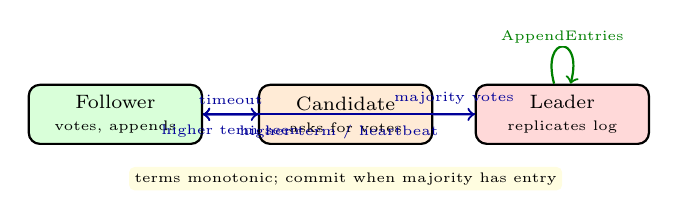
\begin{tikzpicture}[scale=0.86, every node/.style={font=\scriptsize},
  st/.style={draw,rounded corners=4pt,minimum width=2.2cm,minimum height=0.75cm,align=center,thick}]
\node[st,fill=green!15] (foll) at (0,1.6) {Follower\\{\tiny votes, appends}};
\node[st,fill=orange!16] (cand) at (3.4,1.6) {Candidate\\{\tiny asks for votes}};
\node[st,fill=red!15] (lead) at (6.6,1.6) {Leader\\{\tiny replicates log}};
\draw[->,thick,blue!60!black] (foll) -- (cand) node[midway,above,font=\tiny] {timeout};
\draw[->,thick,blue!60!black] (cand) -- (lead) node[midway,above,font=\tiny] {majority votes};
\draw[->,thick,blue!60!black] (cand) -- (foll) node[midway,below,font=\tiny] {higher term seen};
\draw[->,thick,blue!60!black] (lead) -- (foll) node[midway,below,font=\tiny] {higher term / heartbeat};
\draw[->,thick,green!50!black,loop above] (lead) to[loop above] node[font=\tiny,fill=white,inner sep=1pt] {AppendEntries} (lead);
\node[font=\tiny,fill=yellow!12,rounded corners=2pt,inner sep=2pt] at (3.4,0.65) {terms monotonic; commit when majority has entry};
\end{tikzpicture}
\caption{Raft state machine: follower $\to$ candidate on timeout, candidate $\to$ leader on majority, any state $\to$ follower on higher term. Leader replicates log.}
\label{fig:raft-states}
\end{figure}

\begin{figure}[h]
\centering
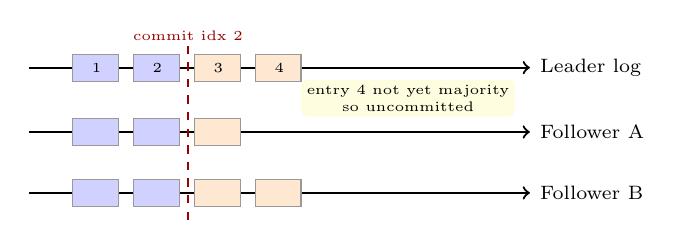
\begin{tikzpicture}[scale=0.86, every node/.style={font=\scriptsize}]
\draw[->,thick] (0,2.0) -- (7.4,2.0) node[right] {Leader log};
\draw[->,thick] (0,1.05) -- (7.4,1.05) node[right] {Follower A};
\draw[->,thick] (0,0.15) -- (7.4,0.15) node[right] {Follower B};
\foreach \x/\c in {1.0/blue!18,1.9/blue!18,2.8/orange!18,3.7/orange!18} \fill[\c,draw=black!40] (\x-0.35,1.80) rectangle (\x+0.32,2.20);
\node[font=\tiny] at (1.0,2.0) {1}; \node[font=\tiny] at (1.9,2.0) {2}; \node[font=\tiny] at (2.8,2.0) {3}; \node[font=\tiny] at (3.7,2.0) {4};
\foreach \x/\c in {1.0/blue!18,1.9/blue!18,2.8/orange!18} \fill[\c,draw=black!40] (\x-0.35,0.85) rectangle (\x+0.32,1.25);
\foreach \x/\c in {1.0/blue!18,1.9/blue!18,2.8/orange!18,3.7/orange!18} \fill[\c,draw=black!40] (\x-0.35,-0.05) rectangle (\x+0.32,0.35);
\draw[thick,red!60!black,dashed] (2.35,-0.25) -- (2.35,2.35) node[above,font=\tiny,fill=white,inner sep=1pt] {commit idx 2};
\node[font=\tiny,align=center,fill=yellow!12,rounded corners=2pt,inner sep=2pt] at (5.6,1.55) {entry 4 not yet majority\\so uncommitted};
\end{tikzpicture}
\caption{Raft log replication: leader appends entries and replicates; entry is committed when a majority stores it (index 2). Uncommitted entries may be overwritten.}
\label{fig:raft-log}
\end{figure}

\begin{lstlisting}[language=Python]
# Raft leader: replicate and commit when majority ack (simplified)
class RaftLeader:
    def __init__(self, n):
        self.n, self.log = n, []          # log is list of (term, cmd)
        self.term = 1
        self.commit_idx = -1
        self.match_idx = [-1]*n           # highest replicated idx per follower
    def append(self, cmd):
        self.log.append((self.term, cmd))
        return len(self.log)-1
    def on_ack(self, follower, idx):
        self.match_idx[follower] = max(self.match_idx[follower], idx)
        # commit if majority has idx and term matches current term
        sorted_match = sorted(self.match_idx + [len(self.log)-1])
        majority_idx = sorted_match[len(sorted_match)//2]
        if majority_idx > self.commit_idx and self.log[majority_idx][0]==self.term:
            self.commit_idx = majority_idx
            print(f"committed up to index {self.commit_idx}: {self.log[:self.commit_idx+1]}")

leader = RaftLeader(5)
leader.append("x:=1"); leader.append("y:=2")
leader.on_ack(1, 1); leader.on_ack(2, 1)  # 3 of 5 have idx 1 -> commit 1
leader.on_ack(3, 0)                        # not enough for idx beyond
\end{lstlisting}

% ============================================================
\section{Byzantine Fault Tolerance}
\label{sec:bft}
When faulty nodes may lie, crash-fault consensus fails. Byzantine agreement needs $n\ge 3f+1$ (Pease--Shostak--Lamport, 1980) and typically $O(n^2)$ messages. PBFT (Castro--Liskov, 1999) is the canonical protocol.

PBFT has three phases per request: \emph{pre-prepare} (primary broadcasts ordering), \emph{prepare} (replicas broadcast that they accept the ordering, $2f$ matching prepares form a prepared certificate), and \emph{commit} ($2f+1$ matching commits guarantee linearizability). A view change replaces a faulty primary. Modern BFT (HotStuff, Tendermint) linearises communication via the leader to reduce messages.

\begin{lstlisting}[language=Python]
# Byzantine quorum intuition: why 3f+1? Two quorums of size 2f+1 overlap in f+1 nodes,
# so even if f of them are Byzantine, at least one honest node is in the overlap.
def quorum_overlap(n, f):
    q = 2*f + 1
    overlap = 2*q - n
    honest_in_overlap = overlap - f      # worst case: f Byzantine in overlap
    return q, overlap, honest_in_overlap

for f in [1,2,3]:
    n = 3*f + 1
    q, ov, hon = quorum_overlap(n, f)
    print(f"f={f} n={n} quorum={q} overlap={ov} honest_in_overlap={hon} (need >=1)")

# With n=3f, overlap=f, honest_in_overlap could be 0 -> safety violated
print("n=3f fails:", quorum_overlap(6, 2))
\end{lstlisting}

\begin{remark}[Paxos vs.\ Raft in practice]
Paxos is more flexible (any proposer, no distinguished leader needed for correctness) but harder to implement correctly; Raft pins leadership to simplify reasoning and adds the election restriction to guarantee leader completeness. Most new systems choose Raft for operability; Paxos variants (EPaxos, WPaxos) win when leader bottlenecks dominate.
\end{remark}

\begin{example}[Raft log matching]
Leader with log $[a_1,b_1]$ and follower with $[a_1]$: the AppendEntries consistency check ($\text{prevLogIndex},\text{prevLogTerm}$) fails for any entry that would diverge, so the leader decrements \texttt{nextIndex} and retries with older entries until the logs align, then overwrites the tail. This is how Raft repairs a follower that missed writes while partitioned.
\end{example}

\begin{remark}[Commit latency]
Consensus latency is at least one round-trip to a majority. Raft batches AppendEntries to amortise this, and followers can serve linearizable reads via a heartbeat round-trip or lease read; otherwise stale reads are faster but may violate linearizability (the read-index optimisation).
\end{remark}

% ============================================================
\section{Exercises}
\label{sec:ch04-exercises}
\begin{enumerate}[label=E4.\arabic*, leftmargin=*, itemsep=0.6em]
    \item \textbf{FLP and timeouts.} State FLP precisely and explain why adding a perfect failure detector would circumvent it. Why is implementing a perfect detector equivalent to solving consensus in async?
    \item \textbf{Paxos trace.} With 3 acceptors, proposer $P_1$ with ballot 1 proposes $v=a$ and reaches only acceptor $A_1$; then $P_2$ with ballot 2 runs Phase~1 contacting $A_2,A_3$. What value must $P_2$ propose? Show the quorum-intersection argument that forces this choice.
    \item \textbf{Raft election.} In a 5-node Raft cluster, follower $F$ has log $[(1,x),(1,y)]$ (last term 1). Candidate $C$ has $[(1,x)]$ and term 2. Can $C$ win election if $F$ is among the voters? State Raft's election restriction and apply it.
    \item \textbf{Commit rule.} Explain why Raft only commits entries from the current term via majority. Give a scenario where committing an old-term entry by counting replicas would violate safety (the figure-8 example in the Raft paper).
    \item \textbf{PBFT quorum.} Prove $n\ge 3f+1$ is necessary for Byzantine agreement with oral messages (sketch the partitioning argument). For $n=7$, what is the largest $f$ tolerated and what quorum size does PBFT use for prepare and commit?
\end{enumerate}

% ============================================================
\section*{Chapter Notes}
Lamport, ``The part-time parliament'' (1998) for Paxos; Paxos Made Simple (2001) is the readable version. Ongaro--Ousterhout, ``In search of an understandable consensus algorithm'' (USENIX ATC, 2014) for Raft. FLP: Fischer--Lynch--Paterson (JACM, 1985). Byzantine generals: Lamport--Shostak--Pease (1982). PBFT: Castro--Liskov (OSDI, 1999). HotStuff: Yin et al.\ (PODC, 2019). For a unified view see Cachin et al., Ch.~5 and Kleppmann Ch.~9.

% End of Chapter 4
